% ----------------------------------------------------------------
\chapter{Methodology / Proposed System}
\section{System Architecture / System Design}
ARC is organised in five layers (Figure~\ref{fig:arch}). At the bottom, a Kubernetes testbed runs the application under test and an open-loop load generator that keeps the offered load constant even when the system slows down. Above it, the experiment harness injects faults, applies remediation actions and plans campaigns. The data pipeline turns the telemetry of each episode into features and damage labels. The ARC layer holds the graph damage model, the dynamic model, the blast-radius explainer and the decision gate. At the top, an interface lets an agent or an engineer ask about a candidate action before it is executed.

\begin{figure}[H]
\centering
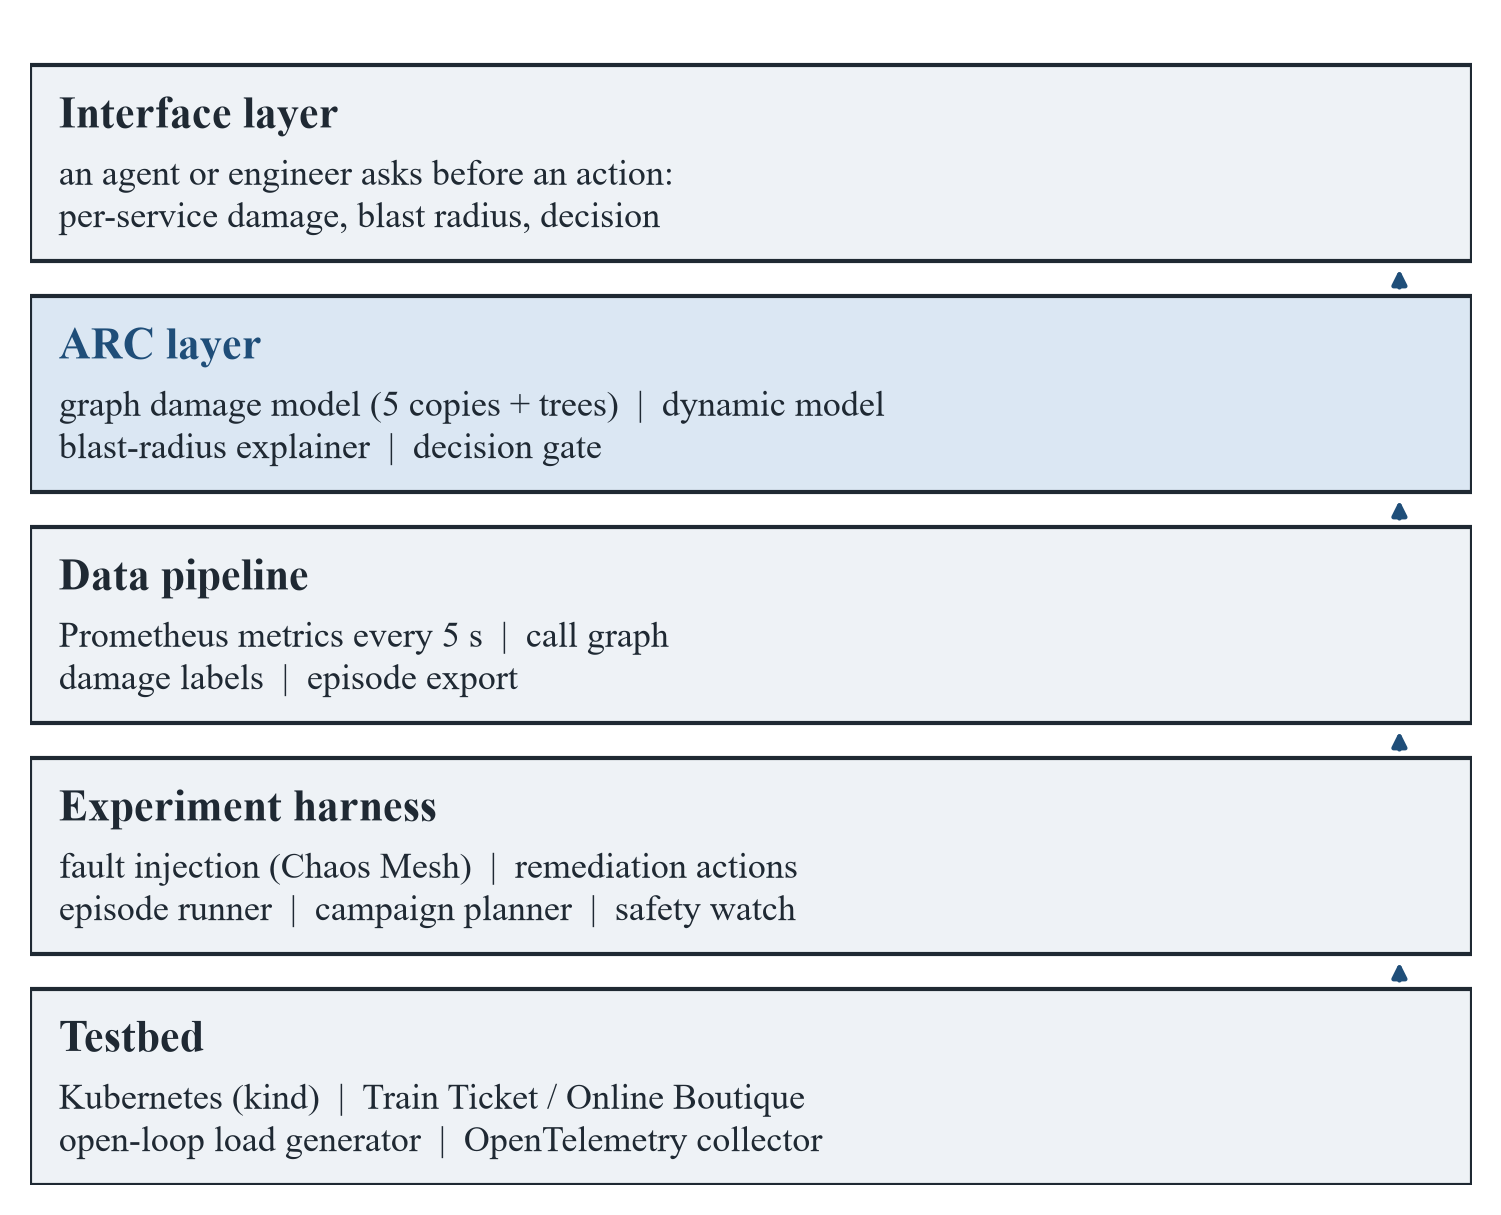
\includegraphics[width=0.82\textwidth]{arch.png}
\caption{Layered architecture of ARC.}
\label{fig:arch}
\end{figure}

Figure~\ref{fig:flow} shows the two flows through this architecture. In the data-collection flow (A) one episode is recorded: the cluster is checked, a 120 s baseline is taken, a fault is injected, the system waits 60 to 300 s, the state of the last 60 s is snapshotted, one random action is applied, and the next 180 s are measured and labelled. Everything the model uses is measured before the action; the label is measured after it. In the decision flow (B) the model reads the same pre-action state and the call graph and scores a candidate action; the damage per service becomes a blast-radius explanation and a decision.

\begin{figure}[H]
\centering
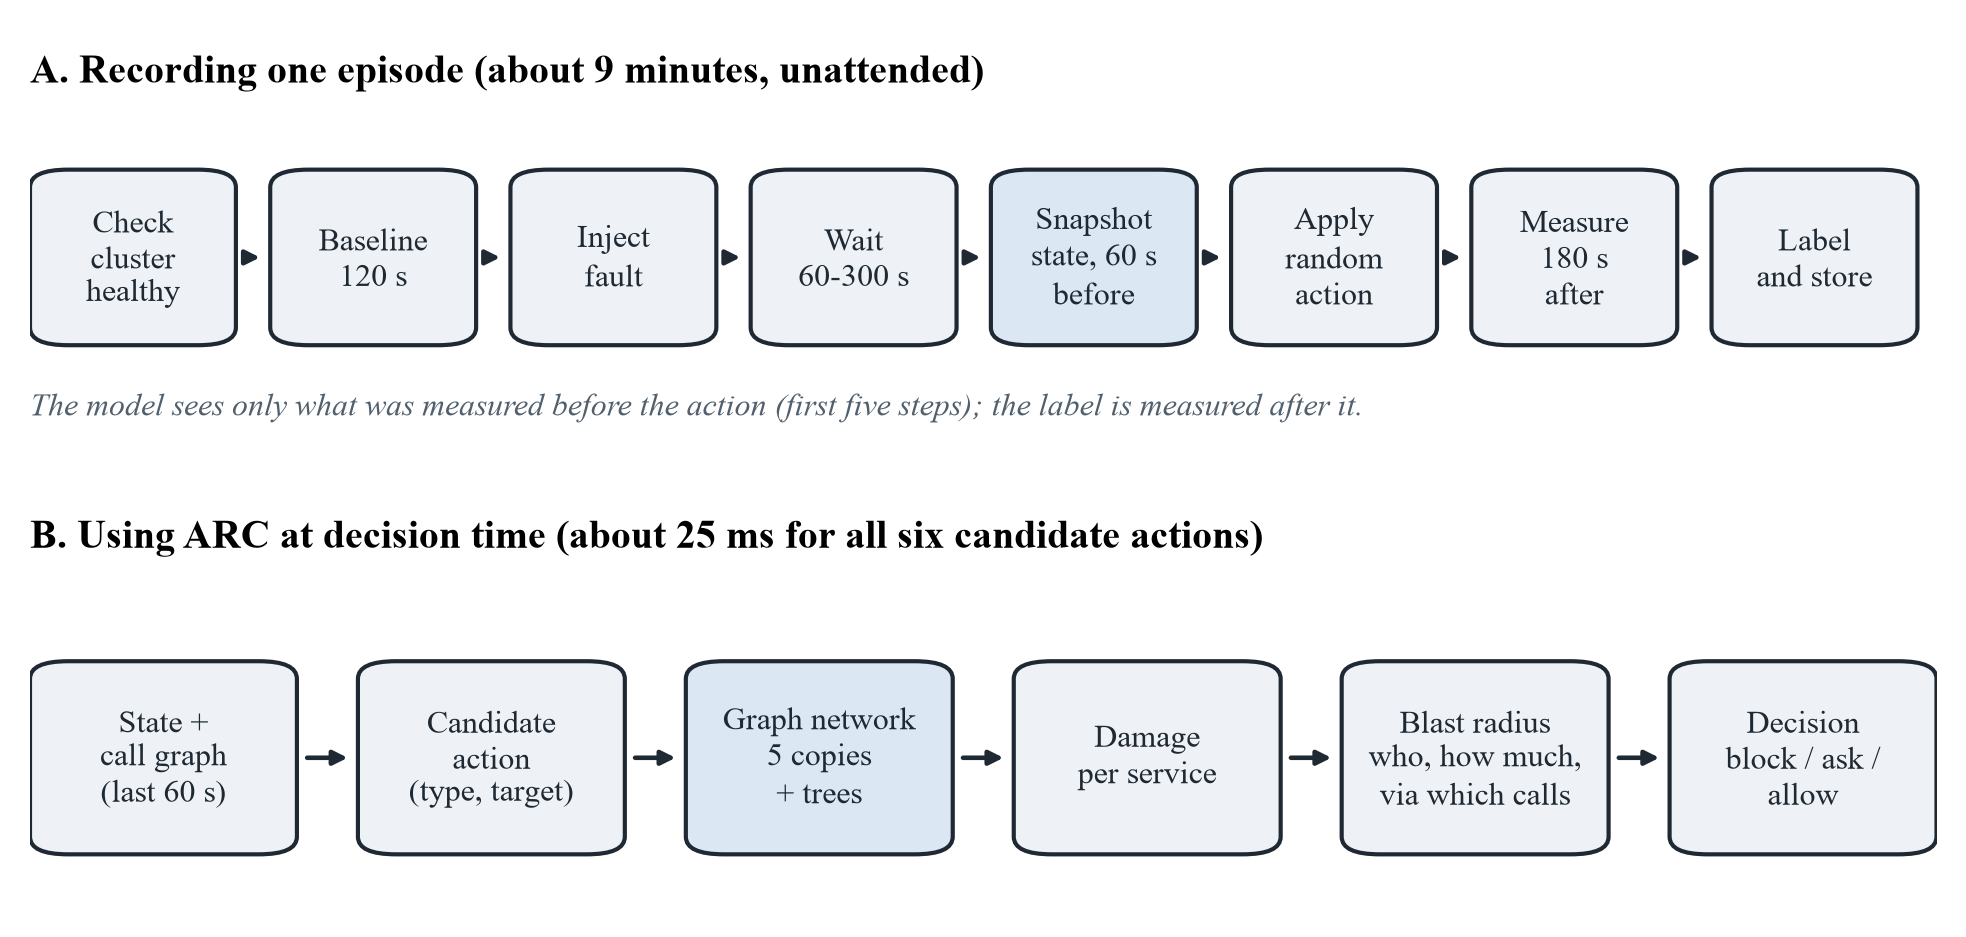
\includegraphics[width=\textwidth]{flow.png}
\caption{Flow chart of the proposed system: (A) recording one episode and (B) using ARC at decision time.}
\label{fig:flow}
\end{figure}

\section{Testbed and Data Collection}
\subsection{Application and infrastructure}
The main application is Train Ticket~[20], a ticket-booking system of 20 services in its core form and 25 in its wide form, written mostly in Java. It runs on Kubernetes 1.34 inside kind on one workstation. OpenTelemetry spans reach Prometheus through the collector, which produces per-service request rates, latency histograms and the service call graph every 5 seconds; cAdvisor and kube-state-metrics supply CPU, memory and readiness. Chaos Mesh~[22] injects the faults. A load generator sends nine kinds of user requests (search, orders, booking, payment, cancel and collection flows) at 4 or 8 requests per second with Poisson arrivals.

\subsection{Faults and actions}
Each episode injects one fault and applies one action 60 to 300 seconds later. Table~\ref{tab:fa} lists the nine fault types and six actions and how often each occurs in the dataset.

\begin{table}[H]
\centering
\caption{Faults and actions in the dataset (episodes).}
\label{tab:fa}
\small
\begin{tabular}{@{}lr@{\hspace{1.2cm}}lr@{}}
\toprule
Fault & Episodes & Action & Episodes \\
\midrule
none & 273 & no-op (control) & 512 \\
packet loss & 467 & restart-pod & 259 \\
network delay & 434 & rollout-restart & 258 \\
pod-kill & 273 & drain & 258 \\
hung pod & 119 & scale-up & 255 \\
CPU squeeze & 61 & cpu-bump & 253 \\
database delay & 63 & & \\
call cut & 63 & & \\
load surge & 42 & & \\
\bottomrule
\end{tabular}
\end{table}

The actions are: \textbf{restart-pod} (delete the pod so that a new one starts), \textbf{rollout-restart} (replace the pod through the deployment), \textbf{scale-up} (add a second copy), \textbf{cpu-bump} (raise the CPU limit in place), \textbf{drain} (take the instance out of rotation without stopping it) and \textbf{no-op} (do nothing; the control). Because the no-op is applied to every fault condition, the damage of an action can be separated from the damage of the fault itself.

\subsection{Campaign design}
A campaign is planned before it runs. It is cut into blocks of seven episodes that share one fault condition: one episode per action, and the no-op twice. Blocks never straddle the split between training and test data. The campaign runs unattended, 6 to 7 episodes per hour, with a health check before each episode, an automatic repeat of an episode that fails, a disk guard and a safety watch. The six parts of the dataset were recorded between 17 and 26 October 2026 on one Intel i9-13900 workstation with 32~GB of memory.

\section{Damage Label}
\subsection{Bad requests and measurement windows}
A request is \emph{bad} if it fails or takes longer than a latency bar. We use three bars: a per-operation bar calibrated on healthy episodes (99th percentile of healthy latency, with a floor of 100~ms), and fixed bars of 500~ms and 1~s. The \emph{bad-request share} of a service in a window is the number of its bad requests divided by all its requests.

For every action, two windows are used (Figure~\ref{fig:windows}). The baseline window $B$ is the 60~s before the action. The measurement window $M$ starts 5~s after the action, lasts 180~s and is divided into six blocks $b_1,\dots,b_6$ of 30~s.

\begin{figure}[H]
\centering
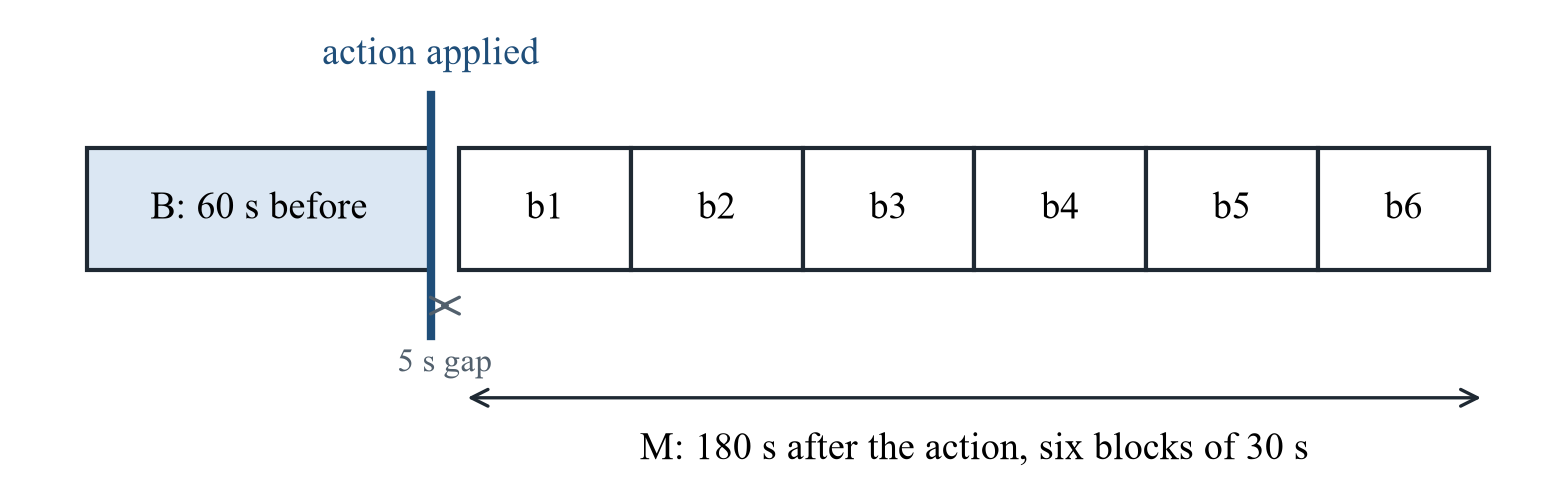
\includegraphics[width=0.95\textwidth]{windows.png}
\caption{Baseline window $B$ and measurement window $M$ around the action.}
\label{fig:windows}
\end{figure}

\subsection{Damage measures}
The \emph{mean damage} of service $i$ is the change of its bad-request share between the two windows:
\begin{equation}
y_i^{\mathrm{mean}} = p_i^{M} - p_i^{B}, \qquad p = \frac{\text{bad requests}}{\text{all requests}}.
\end{equation}
For example, a service that went from 2\% bad requests to 7\% has a mean damage of 5 percentage points (pp). A block with few requests could show exactly 0\% or 100\%, so for the per-block shares half a request is added to the counts:
\begin{equation}
\tilde{p}_{ib} = \frac{\mathrm{bad}_{ib} + 0.5}{n_{ib} + 1}.
\end{equation}
The \emph{peak damage} is the largest increase in any 30-second block, which exposes short, sharp harm that an average hides:
\begin{equation}
y_i^{\mathrm{peak}} = \max_{b=1,\ldots,6}\ \tilde{p}_{ib} - \tilde{p}_i^{B}.
\end{equation}
The \emph{net effect} of an action is the sum of the mean damage over the services with enough traffic, that is at least 30 requests in both windows:
\begin{equation}
\mathrm{net}(a) = \sum_{i \in E} y_i^{\mathrm{mean}}, \qquad E = \{\, i : n_i^{B} \geq 30 \ \text{and}\ n_i^{M} \geq 30 \,\}.
\end{equation}
The net effect gives one score per action, which is what we use to compare actions. The labels also include the time a service takes to return to its baseline.

\subsection{Quality rules}
A service is scored only with 30 or more requests before and after the action. An episode in which at least 80\% of user requests were already bad before the action is flagged as saturated and analysed separately. An episode in which more than a quarter of the measurement window was lost to a machine stall is flagged as stalled. Every incident is repeated across all six actions. The latency bar is calibrated only on healthy no-op episodes: for Train Ticket it was fitted on 12 episodes and checked on 8 that were not used for fitting.

\section{The ARC Dataset}
Dataset v1.0 contains 1,795 campaign episodes in one table with a column that names the part, plus 80 healthy calibration episodes that are used only to fit the latency bars (Table~\ref{tab:parts}). Of the 37,790 labelled (episode, service) rows, 28,769 have enough requests to be scored. The dataset also records 4,696,050 individual user requests.

\begin{table}[H]
\centering
\caption{Parts of dataset v1.0.}
\label{tab:parts}
\small
\begin{tabular}{@{}lrllp{5.2cm}@{}}
\toprule
Part & Episodes & Services & Load & Faults \\
\midrule
batch 1 & 701 & 20 & 4 req/s & none, pod-kill, delay, loss, CPU squeeze \\
wide1 & 500 & 25 & 4 req/s & none, pod-kill, hung pod, delay, loss \\
wide1-db & 126 & 25 & 4 req/s & none, pod-kill, database delay \\
wide2 & 301 & 25 & 8 req/s & none, pod-kill, hung pod, delay, loss \\
repeat test & 20 & 25 & 8 req/s & 4 recipes repeated 5 times \\
held-out & 147 & 25 & 8 req/s & none, pod-kill, call cut (3 links), load surge (3x, 4x) \\
\bottomrule
\end{tabular}
\end{table}

For every episode the raw files are kept: per-service series every 5~s, the call graph with failed calls, exact request and latency-bucket counters, every request the load generator sent, Kubernetes events, the labels and the episode metadata. Any label can therefore be recomputed with another latency bar. The package has a datasheet, a schema description and a loader, checksums for every file, the licences (CC BY 4.0 for the data, MIT for the code), and host names and user paths were removed from the released files. It is prepared for release on Zenodo and Hugging Face.

\section{Damage Model}
\subsection{Input features}
Each service is described by 25 numbers: 13 state values measured in the 60~s before the action, a role code and the action type. The 13 state values are the request rate relative to the service's own healthy baseline, the error share, the 50th, 95th and 99th percentile latency relative to baseline, CPU use as a fraction of the limit, the share of CPU periods throttled, memory relative to baseline, whether the pod was ever not ready, the bad-request share before the action, an indicator that the service is the action target, and the shares of failed incoming and outgoing calls. All are relative to the service's own healthy level or bounded, so they mean the same on every machine, and the fault itself is never an input. The role code states the relation of the service to the action target: target, direct caller, multi-hop caller, callee or unrelated. The action type is one of the six actions.

\subsection{Graph network}
A service's damage depends on its callers and callees, so the model works on the call graph. Each service starts from an embedding of its features $x_i$, role $r_i$ and the action $a$:
\begin{equation}
h_i^{(0)} = \mathrm{ReLU}\big(W_0\,[x_i,\ r_i,\ a]\big),
\end{equation}
a hidden vector of 64 numbers. Three message-passing layers follow (Figure~\ref{fig:mp}). In each layer a service combines its own state with the mean state of its callers and the mean state of its callees, using separate weights for the two directions, and keeps its own state through a residual connection:
\begin{equation}
h_i^{(l+1)} = h_i^{(l)} + \mathrm{ReLU}\Big( W_s\, h_i^{(l)} + W_c\, \overline{h^{(l)}_{\mathrm{callers}(i)}} + W_e\, \overline{h^{(l)}_{\mathrm{callees}(i)}} \Big), \quad l = 0,1,2.
\end{equation}
A small head maps the final vector to the predicted damage of service $i$.

\begin{figure}[H]
\centering
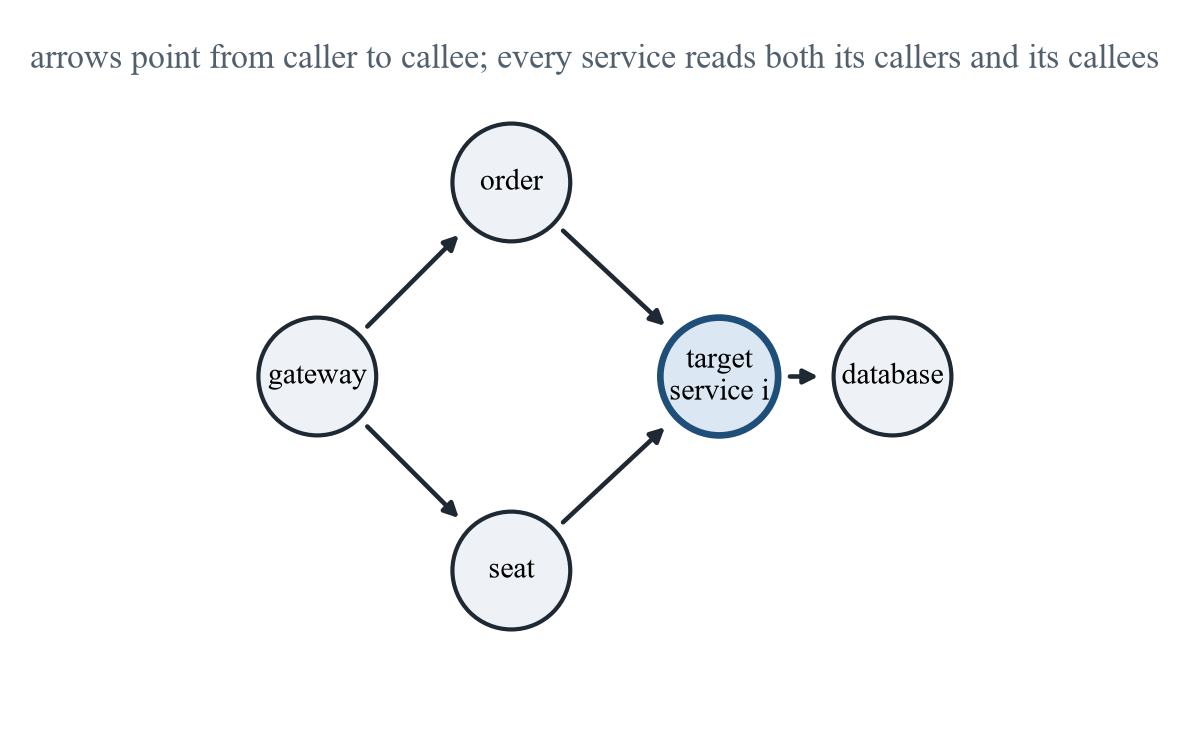
\includegraphics[width=0.78\textwidth]{mp.png}
\caption{Message passing: a service reads the state of its callers and of its callees.}
\label{fig:mp}
\end{figure}

\subsection{Training and final prediction}
The network is trained with the L1 loss (mean absolute error) and the Adam optimiser with early stopping on a validation set made of whole blocks. Five random seeds give five model copies. The final prediction is a weighted ensemble of the graph model and a tree model:
\begin{equation}
\hat{y} = 0.9\,\hat{y}^{\mathrm{GNN}} + 0.1\,\hat{y}^{\mathrm{trees}},
\end{equation}
where $\hat{y}^{\mathrm{GNN}}$ is the mean of the five copies. The spread of the five copies is used as an uncertainty estimate.

\section{Blast Radius, Action Choice and Decision Gate}
\subsection{Blast radius}
Damage spreads through the call graph. Let $d_i(k)$ be the extra bad-request share of service $i$, $k$ steps of 15~s after the action. A linear model fitted on the recorded trajectories describes how it moves:
\begin{equation}
d_i(k{+}1) = a\, d_i(k) + w_{dn}\, \overline{d_{\mathrm{callees}(i)}(k)} + w_{up}\, \overline{d_{\mathrm{callers}(i)}(k)} + g\, d_i(k_a) + u[a, \mathrm{role}_i, k - k_a].
\end{equation}
The fit says that a service keeps most of its own damage ($a = 0.84$) and is pulled by the damage of the services it calls ($w_{dn} = 0.17$) about nine times more than by the services that call it ($w_{up} = 0.02$). The term $g$ is the fault still present at the action, and $u$ is the action's own effect for each role and step. The chain shown to the user is the shortest call path from the target to each service that is hit.

\subsection{Choosing an action}
The same incident is scored six times, once for each candidate action, and the safest action is the one with the lowest predicted net effect:
\begin{equation}
a^{*} = \arg\min_{a \in \mathcal{A}} \widehat{\mathrm{net}}(a), \qquad |\mathcal{A}| = 6.
\end{equation}

\subsection{Decision gate}
The gate turns the predicted net effect and the disagreement of the five copies, $\sigma(a)$, into a decision:
\begin{equation}
\mathrm{decision}(a) =
\begin{cases}
\text{block} & \text{if } \widehat{\mathrm{net}}(a) \geq 20,\\
\text{ask a human} & \text{if } \sigma(a) \geq \sigma_0,\\
\text{allow} & \text{otherwise.}
\end{cases}
\end{equation}
Twenty points of net damage is the blocking threshold. The disagreement threshold $\sigma_0$ is the 90th percentile of the copies' spread on training actions that would not be blocked, so it is set on training data only.

\section{Experimental Setup and Evaluation Protocol}
\subsection{Baselines}
ARC is compared with: \textbf{no damage} (predict zero), a \textbf{runbook average} (the average damage seen for the same action), a \textbf{role rule} (the average damage for the service's role relative to the target), a \textbf{dependency map} (damage assigned to services connected to the target in the call graph), \textbf{tree-based} models, a harmed-or-not \textbf{classifier}, and an \textbf{LLM judge} that is asked to estimate the damage. All baselines were reimplemented and evaluated on the same data and split as ARC.

\subsection{Metrics}
The main metric is the mean absolute error (MAE) between the predicted and the measured damage, in percentage points, on scored services; lower is better. We also report how often the most damaged service is identified, the Spearman rank correlation between predicted and measured damage over all services (1 means identical order), the F1 score for harmed-or-not (a balance of missed harm and false alarms), the share of action pairs ranked correctly, and the block rate of the gate.

\subsection{Protocols}
Six protocols test different kinds of change.
\begin{itemize}
\item \textbf{In-system:} every fifth block of each plan is test data (5-fold); new incidents on the same system.
\item \textbf{Unseen system:} train on batch 1 (20 services), test on wide1 (25 services, 5 of them new).
\item \textbf{Unseen fault:} train on wide1, test on wide1-db (a slow database never seen in training).
\item \textbf{Held-out faults:} train on everything except the held-out part, test on call cuts and load surges that were never seen.
\item \textbf{Higher load:} train on the 4 req/s parts, test on wide2 (8 req/s).
\item \textbf{Noise ceiling:} the same incident repeated five times, to measure the floor on any error.
\end{itemize}

\section{Results}
\subsection{Damage prediction}
Table~\ref{tab:main} and Figure~\ref{fig:results} give the error of ARC and of the best baseline in each protocol. ARC cuts the error roughly in half in every test.

\begin{table}[H]
\centering
\caption{Prediction error (MAE, percentage points; lower is better).}
\label{tab:main}
\small
\begin{tabular}{@{}lccl@{}}
\toprule
Test & ARC & Best baseline & What changes \\
\midrule
In-system (5-fold) & 1.98 & 3.86 (role rule) & new incidents, same system \\
Unseen system & 2.86 & 3.91 (trees) & 20 to 25 services \\
Unseen fault & 1.86 & 2.61 (trees) & slow database, never seen \\
Higher load, wide2 first half & 2.78 & 4.11 (trees) & 4 to 8 requests per second \\
Higher load, all wide2 (1 s bar) & 2.12 & 4.17 (role rule) & 4 to 8 requests per second \\
\bottomrule
\end{tabular}
\end{table}

\begin{figure}[H]
\centering
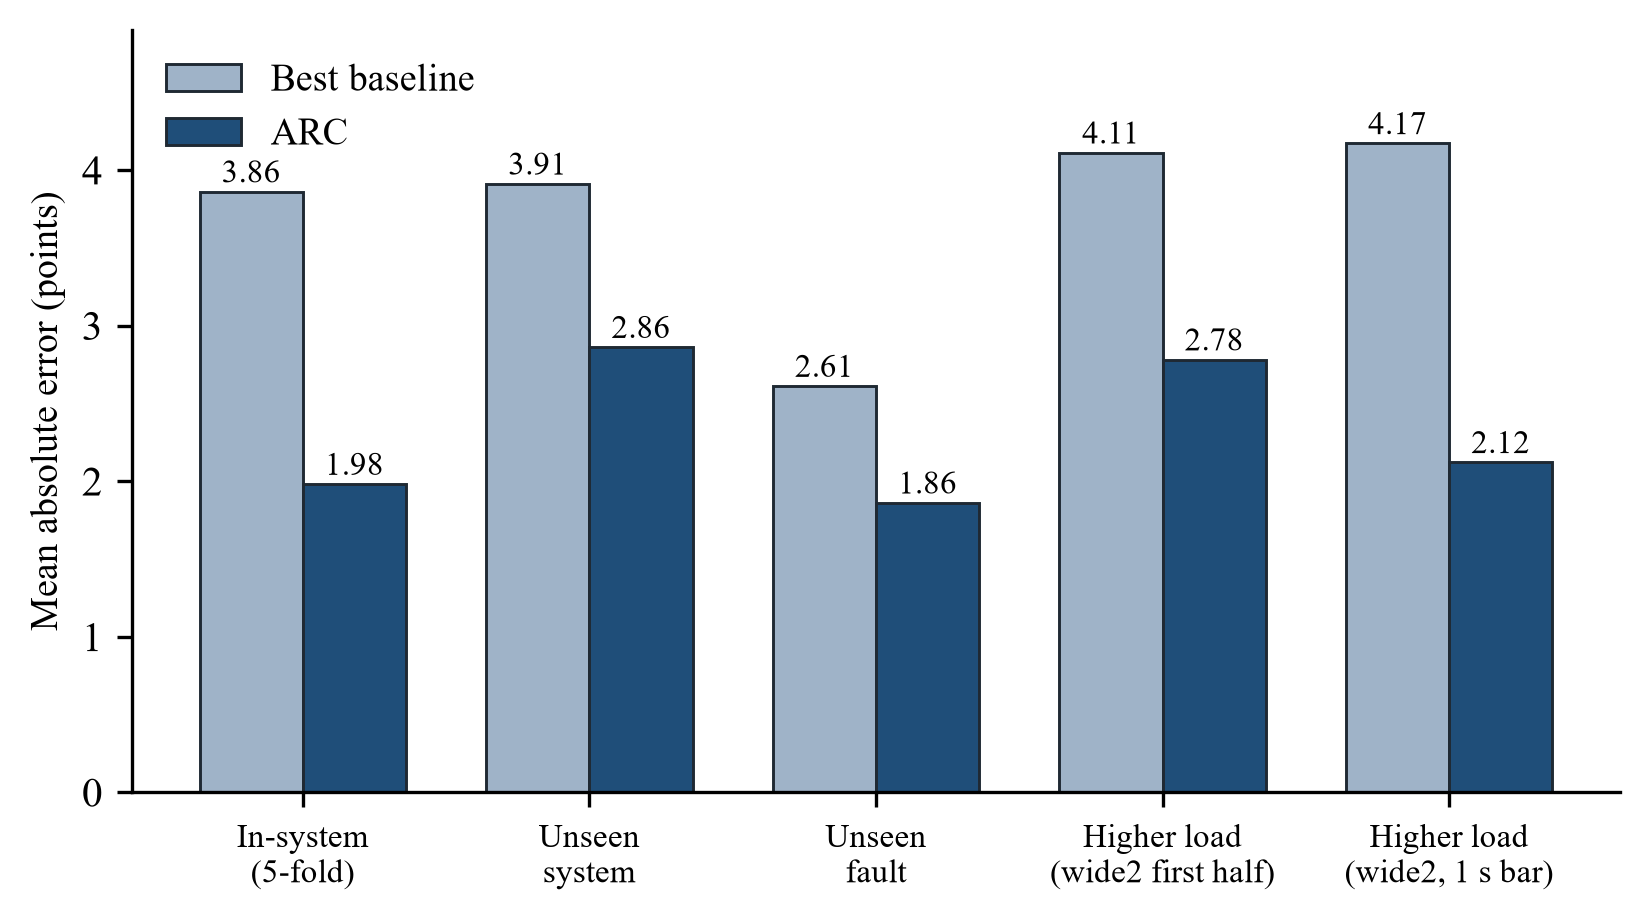
\includegraphics[width=0.92\textwidth]{results.png}
\caption{ARC against the best baseline in five tests.}
\label{fig:results}
\end{figure}

ARC identifies the most damaged service in 78\% of incidents, against 40\% for trees. The trees, however, rank all services better (Spearman correlation 0.75 against 0.68), so ARC does not win on every metric. For harmed-or-not classification ARC reaches an F1 score of 0.77 against 0.75 for the classifier. Across latency bars from 50~ms to 1~s, ARC's error is 0.21 to 0.56 times the error of predicting no damage. On the batch-1 test split alone, ARC's error is 1.83 against 6.46 for the dependency map and 9.03 for the runbook average.

\subsection{Held-out faults and the noise floor}
Table~\ref{tab:held} and Figure~\ref{fig:held} show ARC on 147 episodes of fault types that were not in the training data. ARC is accurate on call cuts and no-fault episodes, but the average is dominated by the four-times traffic surge (error 22.16), a fault of a new kind with no failing component, which the model does not predict. Over all held-out episodes the error is 7.57, level with the best baseline (role rule, 7.51) and below predicting no damage (9.21).

\begin{table}[H]
\centering
\caption{ARC on conditions never seen in training.}
\label{tab:held}
\small
\begin{tabular}{@{}lccc@{}}
\toprule
Condition & Episodes & ARC error & Worst service hit (share bad) \\
\midrule
call cut ts-assurance-service & 21 & 0.98 & 36\% \\
call cut ts-config-service & 21 & 4.65 & 67\% \\
call cut ts-order-other-service & 21 & 3.24 & 40\% \\
traffic surge 3x & 21 & 6.09 & 33\% \\
traffic surge 4x & 21 & 22.16 & 40\% \\
no fault & 21 & 3.20 & 44\% \\
pod-kill & 21 & 5.51 & 41\% \\
\textbf{all held-out} & \textbf{147} & \textbf{7.57} & \textbf{42\%} \\
\bottomrule
\end{tabular}
\end{table}

\begin{figure}[H]
\centering
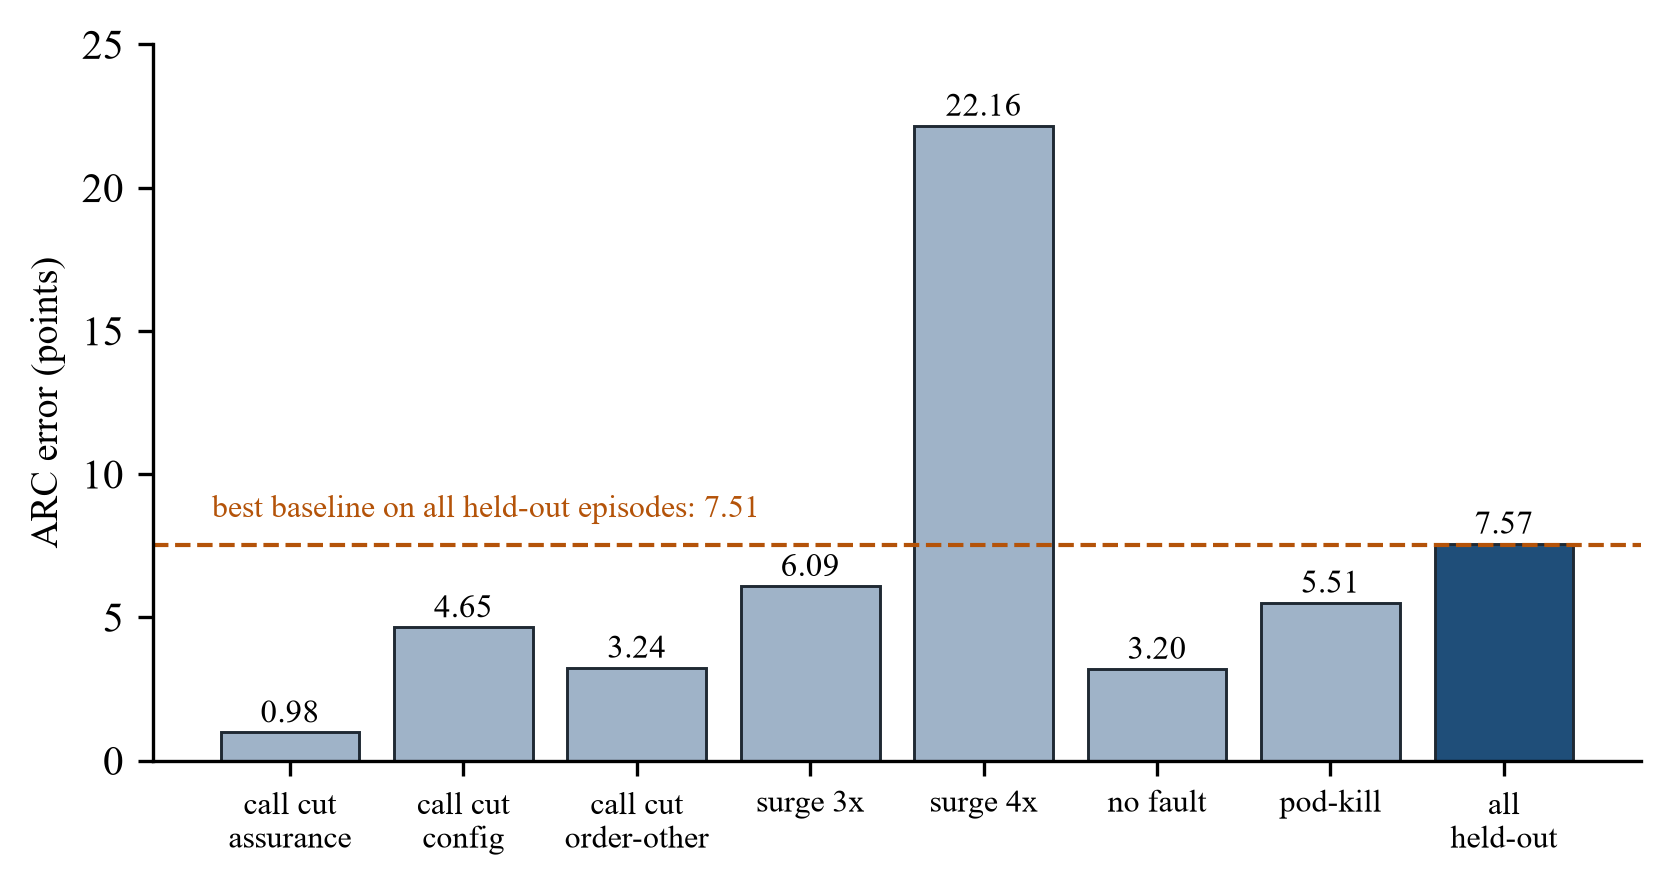
\includegraphics[width=0.92\textwidth]{heldout.png}
\caption{ARC error on conditions never seen in training.}
\label{fig:held}
\end{figure}

The same incident repeated five times does not give the same numbers: total damage varies by 12 to 27\%. No predictor can therefore score below 3.08 points on these incidents; ARC is 2.1 points above this floor and the trees are 7.2 points above it.

\subsection{Uncertainty, speed and decisions}
\textbf{Uncertainty.} When the five model copies disagree the prediction is more often wrong. In the 20\% of episodes with the highest disagreement the error is 3.7 against 1.3 (in-system), 7.2 against 2.0 (unseen system) and 4.5 against 1.2 (unseen fault).

\noindent\textbf{Speed.} The model scores one action in 4~ms and all six in about 25~ms; the full tool takes about 350~ms before optimisation. The LLM judge needs 3.6~s and is no better than predicting no damage.

\noindent\textbf{Explanation, ranking and gate.} The blast-radius explanation reaches a hit-set F1 of 0.74, against 0.64 for a dependency map. Ranking the six actions by predicted net damage puts 86\% of action pairs in the right order, against 80\% for a runbook-style average. The gate blocks 1.6\% of safe actions and detects 84\% of harmful ones.

\section{Validation and Known Limits of the Data}
\textbf{What has been checked.} (i) The latency bar was fitted on healthy episodes only and checked on healthy episodes that were not used to fit it (Train Ticket: fitted on 12, checked on 8). (ii) Labels are reported at three bars, so the results do not depend on one threshold. (iii) Repeating the same incident gives the measurement noise (12 to 27\%, floor 3.08). (iv) Plans, discard rules and scoring rules were fixed before the runs and are applied by code. (v) Every released file has a checksum, the archives pass a gzip test, the loader returns the expected counts for every split, and a scan found no host names or user paths in the released files.

\noindent\textbf{Known issues.} The datasheet lists them; the ones that change results are:
\begin{enumerate}
\item \textbf{Saturation.} In 389 of 1,795 episodes users were already at least 80\% bad before the action. They are flagged and should be excluded, or the 1~s bar used, when ranking actions.
\item \textbf{Drift in wide2.} Two tables read by the cancel flow were not cleaned, so the cancel flow slowed from 77 to 131~ms during wide2. Labels after block 24 are inflated for that flow; the first half of wide2 or the 1~s bar should be used.
\item \textbf{One system, one machine, one copy per service.} Fault levels were dosed on this machine and are not a measure of severity.
\item \textbf{Short bursts are invisible.} The label averages over 180~s; a burst of a few seconds stays in the raw requests only.
\end{enumerate}

\noindent\textbf{What has not been done yet.} The labels measure what the users see (the share of bad requests); no operator has judged whether a given rise matters. All data of version 1.0 was recorded on one machine with one pipeline, so independent replication is still open. Further validity tests (dose--response of the fault levels, agreement of the service-side counters with the load generator's own log, and a check of damage against the call graph) are planned.

\section{Second Application: Online Boutique}
To test whether the pipeline works beyond one application, the testbed was ported to Online Boutique, a Google demonstration shop of 11 services and a cache. The port needed several changes. Three services (ad, cart and shipping) are written in Go, C\# and Java and emit no server-side spans, so they are named through the service graph from their callers' client spans and their labels are computed from the callers' view of the calls (caller view, threshold 100~ms). Draining a service is done with a Chaos Mesh network partition because Online Boutique has no service registry. A restart whose effect lasts about 10~s is invisible in a 180~s label. The latency bar was calibrated at 8 requests per second on healthy episodes (0 false harms in 42 held-out service verdicts, and every service receives a verdict).

A campaign of 280 episodes (40 blocks of 7, eight fault conditions, six actions) was planned in advance. \todo{At the time of writing about 200 of the 280 planned episodes were recorded; insert the final counts before submission.} Two harness faults were found by the safety rules and fixed during the run: a failed drain left its network partition behind, and a CPU squeeze that was followed by a scale-up left a pod throttled; five episodes affected by the second fault are kept but excluded. Saturation in this campaign (about 21\% of episodes) comes only from network delay and hung pods, which is a finding about those faults; packet loss, CPU squeeze, pod-kill and no-fault episodes were never saturated. The no-op control is clean (5 harm rows of 618 service rows), and drain is the most harmful action, as expected. The Online Boutique results are therefore treated as a replication with stated limits, and Train Ticket remains the main benchmark.
